\documentclass{home_assignment}
\usepackage[acronym,nogroupskip]{glossaries}
\usepackage[hidelinks]{hyperref}
\makeglossaries
\newacronym{it}{IT}{Information Technology}
\newacronym{ict}{ICT}{Information and Communication Technology}
\newacronym{gdp}{GDP}{Gross Domestic Product}
\newacronym{aws}{AWS}{Amazon Web Services}
\newacronym{gcp}{GCP}{Google Cloud Platform}
\newacronym{gea}{GEA}{Government Enterprise Architecture}
\newacronym{un}{UN}{United Nations}
\newacronym{ibm}{IBM}{International Business Machines Corporation}
\newacronym{ngo}{NGO}{Non-Governmental Organization}
\newacronym{www}{WWW}{World Wide Web}
\newacronym{ntc}{NTC}{Nepal Telecom}
\newacronym{egmp}{eGMP}{e-Governance Master Plan}
\newacronym{ftth}{FTTH}{Fiber to the Home}
\newacronym{atm}{ATM}{Automated Teller Machine}
\newacronym{abbs}{ABBS}{Any Branch Banking Service}
\newacronym{isp}{ISPs}{Internet Service Providers}
\newacronym{pan}{PAN}{Permanent Account Number}
\newacronym{g2c}{G2C}{Government to Citizen}
\newacronym{g2b}{G2B}{Government to Business}
\newacronym{g2e}{G2E}{Government to Employees}
\newacronym{g2g}{G2G}{Government to Government}
\newacronym{hlcit}{HLCIT}{High Level Commission of Information and Technology}
\newacronym{dbms}{DBMS}{Database Management System}
\newacronym{nitc}{NITC}{National Information Technology Center}
\newacronym{moest}{MoEST}{Ministry of Education, Science and Technology}
\newacronym{moic}{MoIC}{Ministry of Information and Communications}
\newacronym{moga}{MoGA}{Ministry of General Administration}
\newacronym{mof}{MoF}{Ministry of Finance}
\newacronym{eta}{ETA}{Electronic Transaction Act}   
\newacronym{itu}{ITU}{International Telecommunication Union}  
\newacronym{egdi}{EGDI}{e-Government Development Index}
\newacronym{covid}{COVID-19}{Corona Virus Disease of 2019}
\begin{document}
\titlePage{Enterprise Computing Assignment \#1}{June 21, 2021}{Basanta Joshi, Ph.D.\\Dipak Poudel}   
\pagenumbering{roman}
\tableofcontents
\clearpage
\phantomsection
\addcontentsline{toc}{section}{\bfseries{List of Figures}}
\listoffigures
\clearpage
\phantomsection
\addcontentsline{toc}{section}{\bfseries{List of Abbreviations}}
\printglossary[type=\acronymtype,nonumberlist,title={List of Abbreviations}]
\clearpage
\pagenumbering{arabic}
\section{Cloud Computing}
The on-demand delivery of \acrfull{it} resources over the shared internet is known as cloud computing. It is a concept that allows outsourcing of different \acrshort{it} resources such as storage, processing capabilities, or even software via the network that uses the pay-as-you-go model. Advancements in cloud computing have allowed users to shift away from buying and maintaining the data centers, servers, and other resources to accessing such resources as per their requirement from cloud vendors such as \acrfull{aws}, Microsoft Azure, \acrfull{gcp}. Different sized organizations in the industry are turning their heads towards cloud computing for use cases that range from disaster recovery, data backup, virtual desktop environments to big data analysis and software development.

\subsection{Types of Cloud Computing Model}
\subsubsection{Infrastructure as a Service (IaaS)}
\acrfull{iaas} cloud computing model provides computing infrastructure such as servers, network equipment, storage, operating systems through a technology called virtualization. This allows clients that buy \acrshort{iaas} on-demand services complete control over the bought infrastructure such that they don't have to think about maintaining the actual physical hardware. It is the most flexible model as clients have complete control over their infrastructure while still employing the pay-as-yo-go model. \acrfull{aws}, \acrfull{gce} are some common examples.
\subsubsection{Platform as a Service (PaaS)}
\acrfull{paas} cloud computing model provides platform for software creation over the internet. This allows the client company to let its developers focus on software development such that they don't have to focus on the underlying operating system, or any infrastructure. It also provides different kinds of services that are helpful for development and testing of applications. AWS Elastic Beanstalk, Heroku are some common examples.  
\subsubsection{Software as a Service (SaaS)}
\acrfull{saas} cloud computing model provides cloud applications managed by third-party distributors over the internet. Mostly small companies and short-term projects that are looking for instant \acrshort{it} solutions use \acrshort{saas}. Dropbox, Google Workspace, and GoToMeeting are some common examples.
\subsection{Benefits of Cloud Computing}
\subsubsection{Variable Expense}
Companies that employ their services using cloud services trade the overhead cost of buying and maintaining infrastructures with variable expense with the pay-as-you-go model.

\subsubsection{On-demand Scaling of Resources}
Clients can avoid under or over estimating the capacity they need and move towards a better scaled resources using auto scaling services. 

\subsubsection{Increased Speed of Deployment}
Since the \acrshort{it} resources required are available at the push of a button, the deployment process is greatly sped up. 

\subsubsection{Economies of Scale}
With the increase in number of users, the proportional cost saving using the pay-as-you-go model drastically increases. 

\subsubsection{Global Reach without much Hassle}
Clients can deploy their applications to multiple \acrshort{aws} regions without much hassle. This improves their global reach and they can have servers in different geographical regions up and running in few minutes. This ensures low latency for the application hence boosting consumer experience. 

\subsubsection{No Maintenance Cost}
Clients can focus on the delivery of their applications rather than maintaining the infrastructure that are essential. This greatly reduces their maintenance expenditure.

\section{AWS Global Infrastructure}
In order to deliver highly reliable, scalable cloud services over a secure connection, Amazon has segregated it's global infrastructures with 81 availability zones in 25 actual global regions around the globe.
\subsection{AWS Regions}
These are physical geographical locations where data replication across regions depends on the clients need. Currently there are 25 \acrshort{aws} regions that themselves house one or more availability zones. Each region is completely independent of one another and pricing vary in these regions.
\subsection{Availability Zones}
These are isolated AWS infrastructures inside an AWS region that are connected via high bandwidth private networks. Currently there are 81 availability zones that themselves house one or more data centers. The availability zones ensure isolation from natural calamities. 21 new availability zones in 7 \acrshort{aws} regions have been announced recently.
\subsection{Data Centers}
These are physical data centers that store the actual data. Clients can't select data centers instead can select availability zones to deploy their application.

\section{Amazon Elastic Compute Cloud (EC2)} 
\acrfull{ec2} is a service available on the Amazon console dashboard that allows clients to create virtual machines, generally known as \acrshort{ec2} instances. In terms of cloud computing types, an \acrshort{ec2} can be regarded as an \acrshort{iaas} since the client can choose the \acrshort{ami}, and capacity of servers. The said \acrshort{ec2} instances allow clients to host virtual machines on which they can deploy applications in somewhat a similar fashion as an on-premise environment. Few use-cases where \acrshort{ec2} instances are used are as application, web, game, media, mail, database servers. \acrshort{ec2} instances can be launched in the different possible availability zones. The breakdown for Amazon \acrshort{ec2} is as,
\begin{itemize}
    \item \textbf{Elastic :} Since number of instances can be auto-scaled.
    \item \textbf{Compute :} Since most use-cases of \acrshort{ec2} include the use of compute resources.
    \item \textbf{Cloud :} Since \acrshort{ec2} instances are available as cloud service.
\end{itemize}


\subsection{Choose an Amazon Machine Image}
\begin{figure}[H]
    \centering
    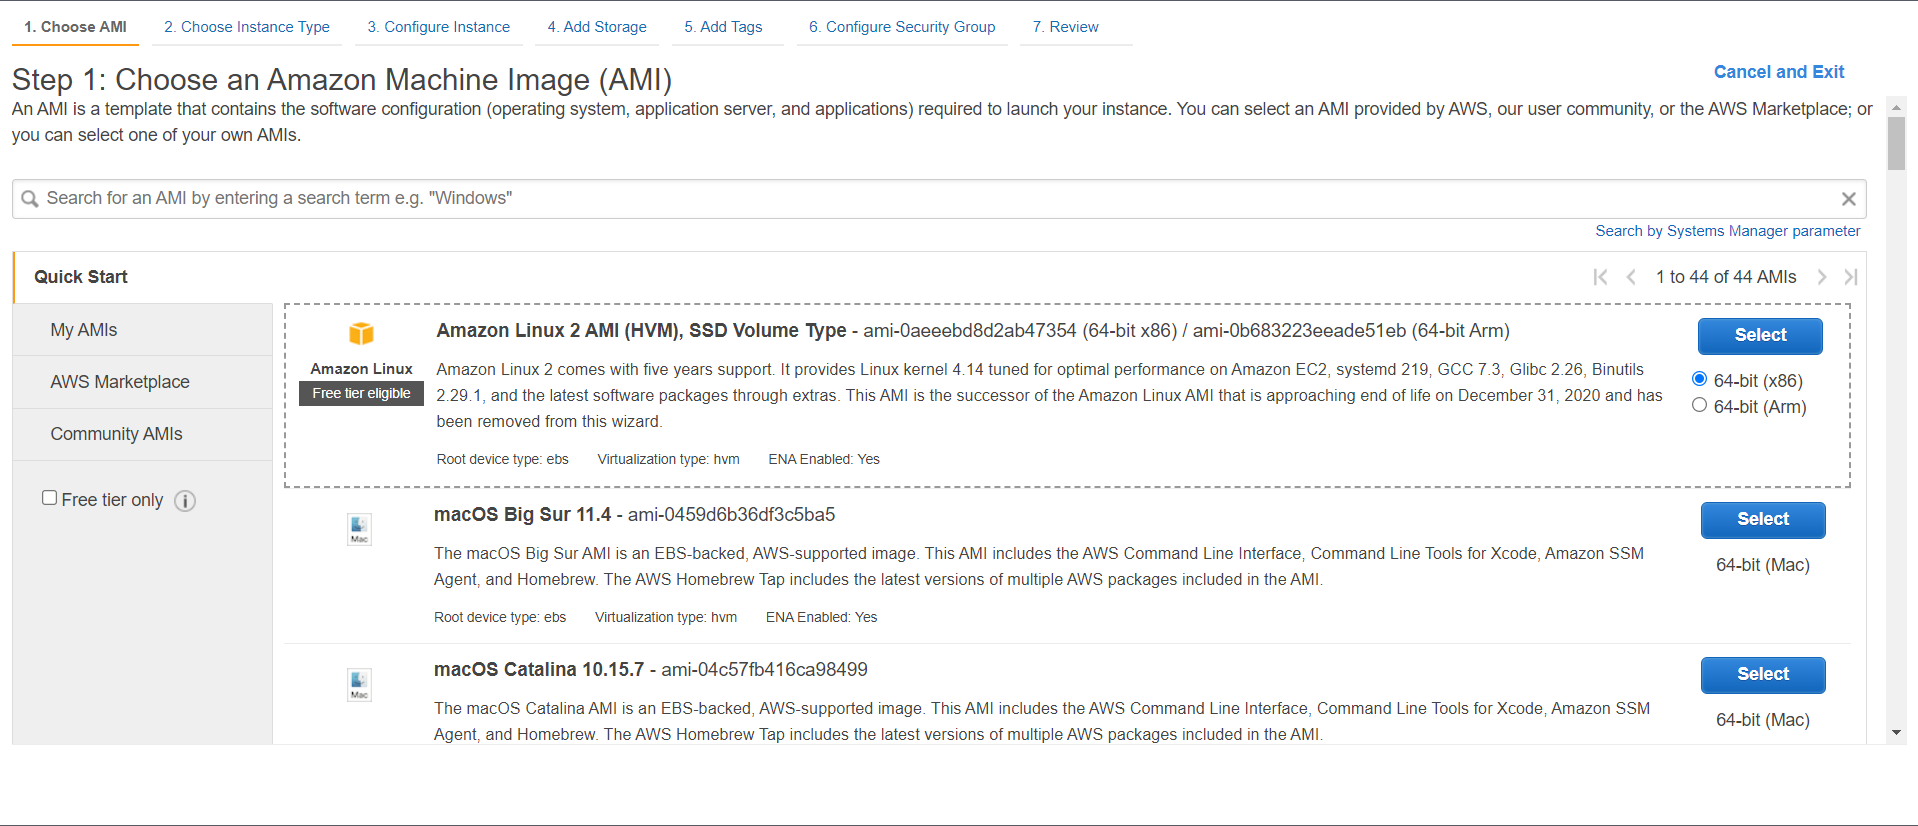
\includegraphics[frame,width=\linewidth]{../Figures/a.png}
    \label{fig:a}
    \caption{Choose an \acrlong{ami}}
\end{figure}
This is the first step in creation of an \acrshort{ec2} instance. This step involves selection of an \acrshort{ami} based on which the desired \acrshort{ec2} instance is created. \acrfull{ami} is an image that contains the configurations such as operating system, required application servers. \acrshort{aws} allows selection of \acrshort{ami} provided by \acrshort{aws}, or the ones created by the vast user community or some available on the \acrshort{aws} marketplace. For this example, Amazon Linux is selected as the \acrshort{ami}.


\subsection{Choose an Instance Type}
\begin{figure}[H]
    \centering
    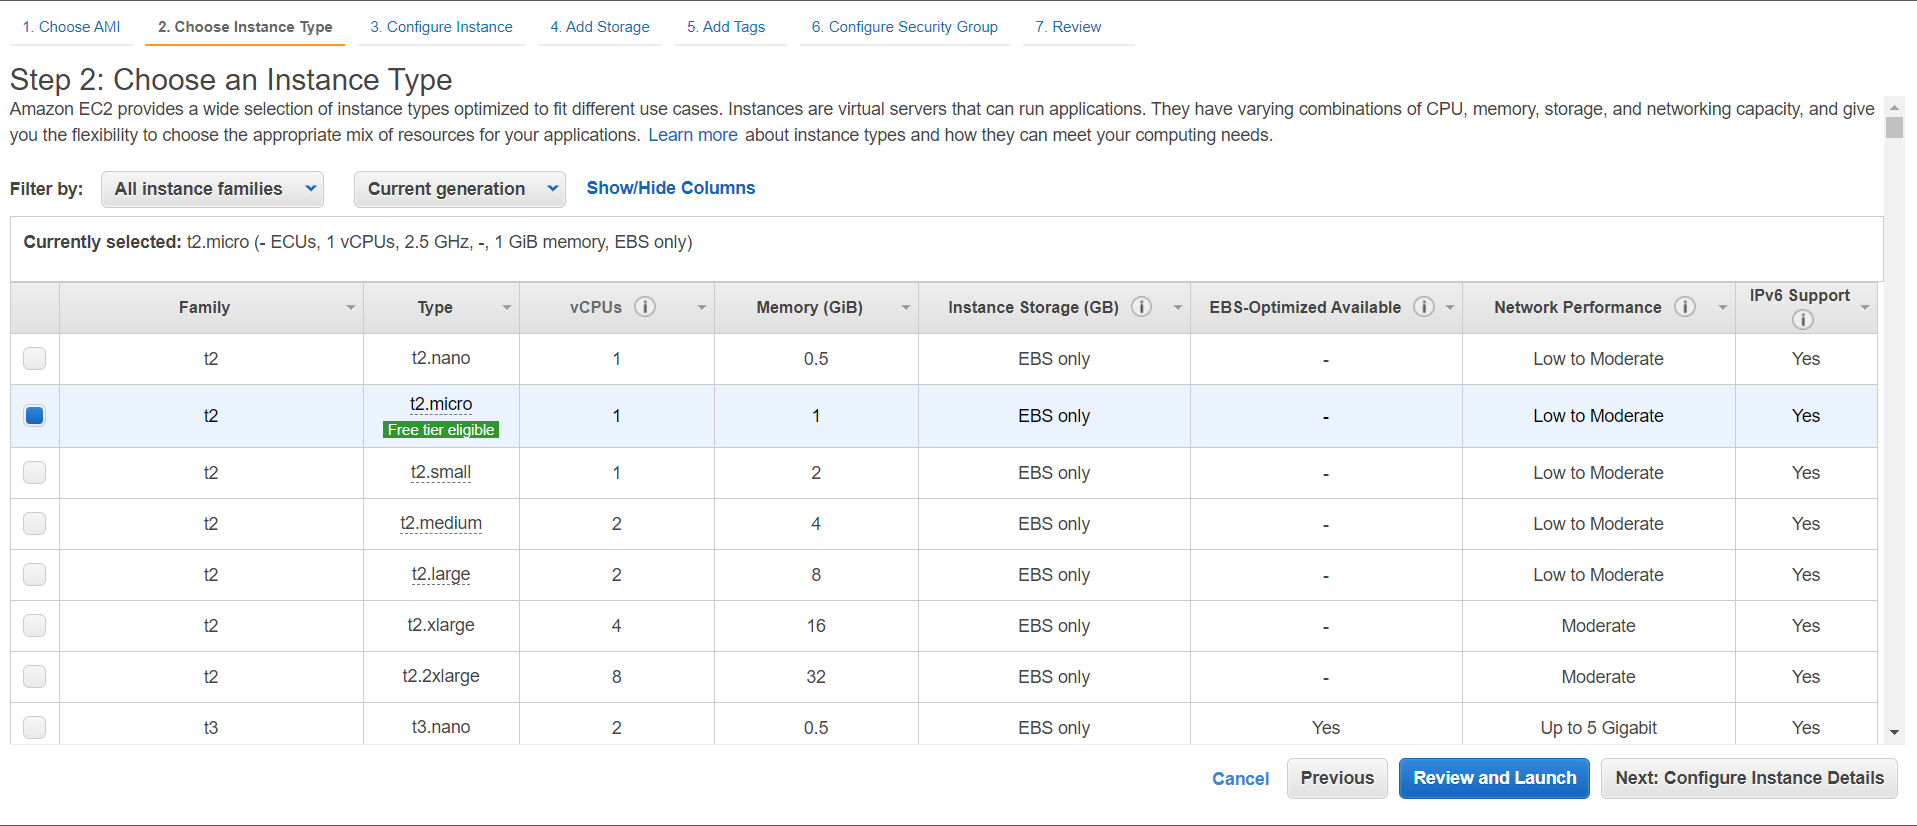
\includegraphics[frame,width=\linewidth]{../Figures/b.png}
    \label{fig:b}
    \caption{Choose an Instance Type}
\end{figure}
This is the second step in creation of an \acrshort{ec2} instance. This step involves selection of an \acrshort{ec2} types based on which the desired combination of CPU, storage, network performance, memory other resources are set. \acrfull{ec2} instance types provide different optimal combinations out of which \textit{t2.micro}, a free tier type is selected for this example. The \textit{t2.micro} instance type provides 1 vCPU, 1 GiB memory, low to moderate network performance and \acrshort{ebs} storage support.

\subsection{Configure Instance Details}
\begin{figure}[H]
    \centering
    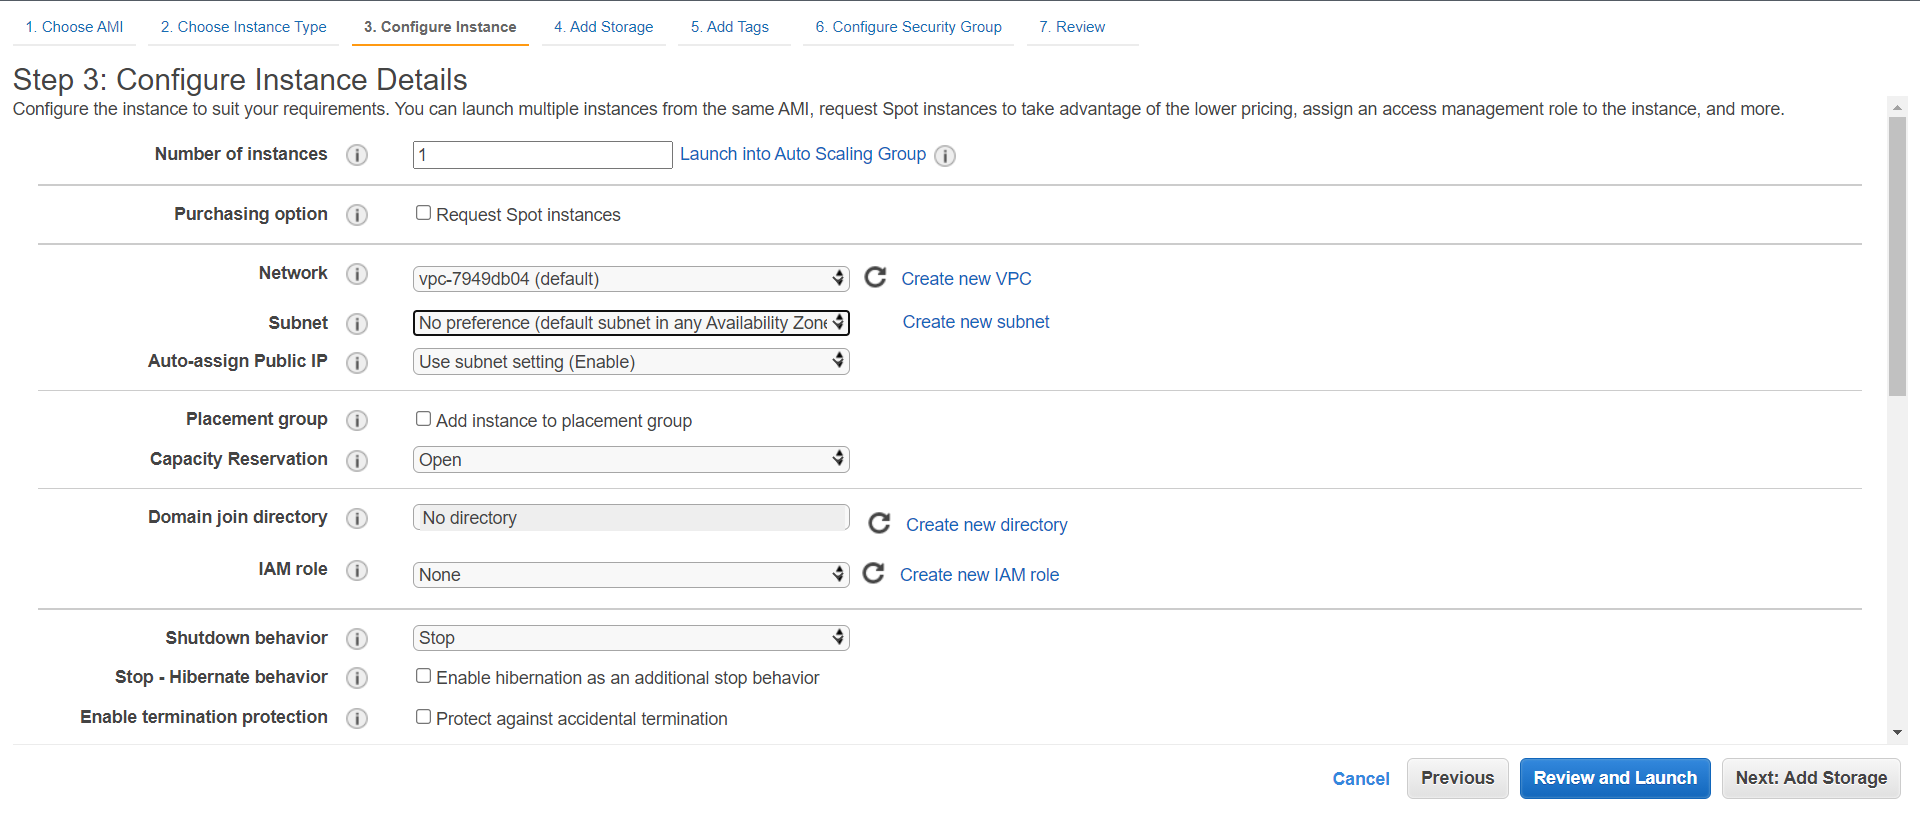
\includegraphics[frame,width=\linewidth]{../Figures/c.png}
    \label{fig:c}
    \caption{Configure Instance Details}
\end{figure}
This is the third step in creation of an \acrshort{ec2} instance. This step involves configuration of the \acrshort{ec2} instance details. Configuration options such as number of instances under the same \acrshort{ami}, different purchasing options, network settings for \acrshort{vpc} creation and setting subnets, \acrshort{iam} roles, behavior on shutdown and hibernation can be set using this step of instance launch.

\subsection{Add Storage}
\begin{figure}[H]
    \centering
    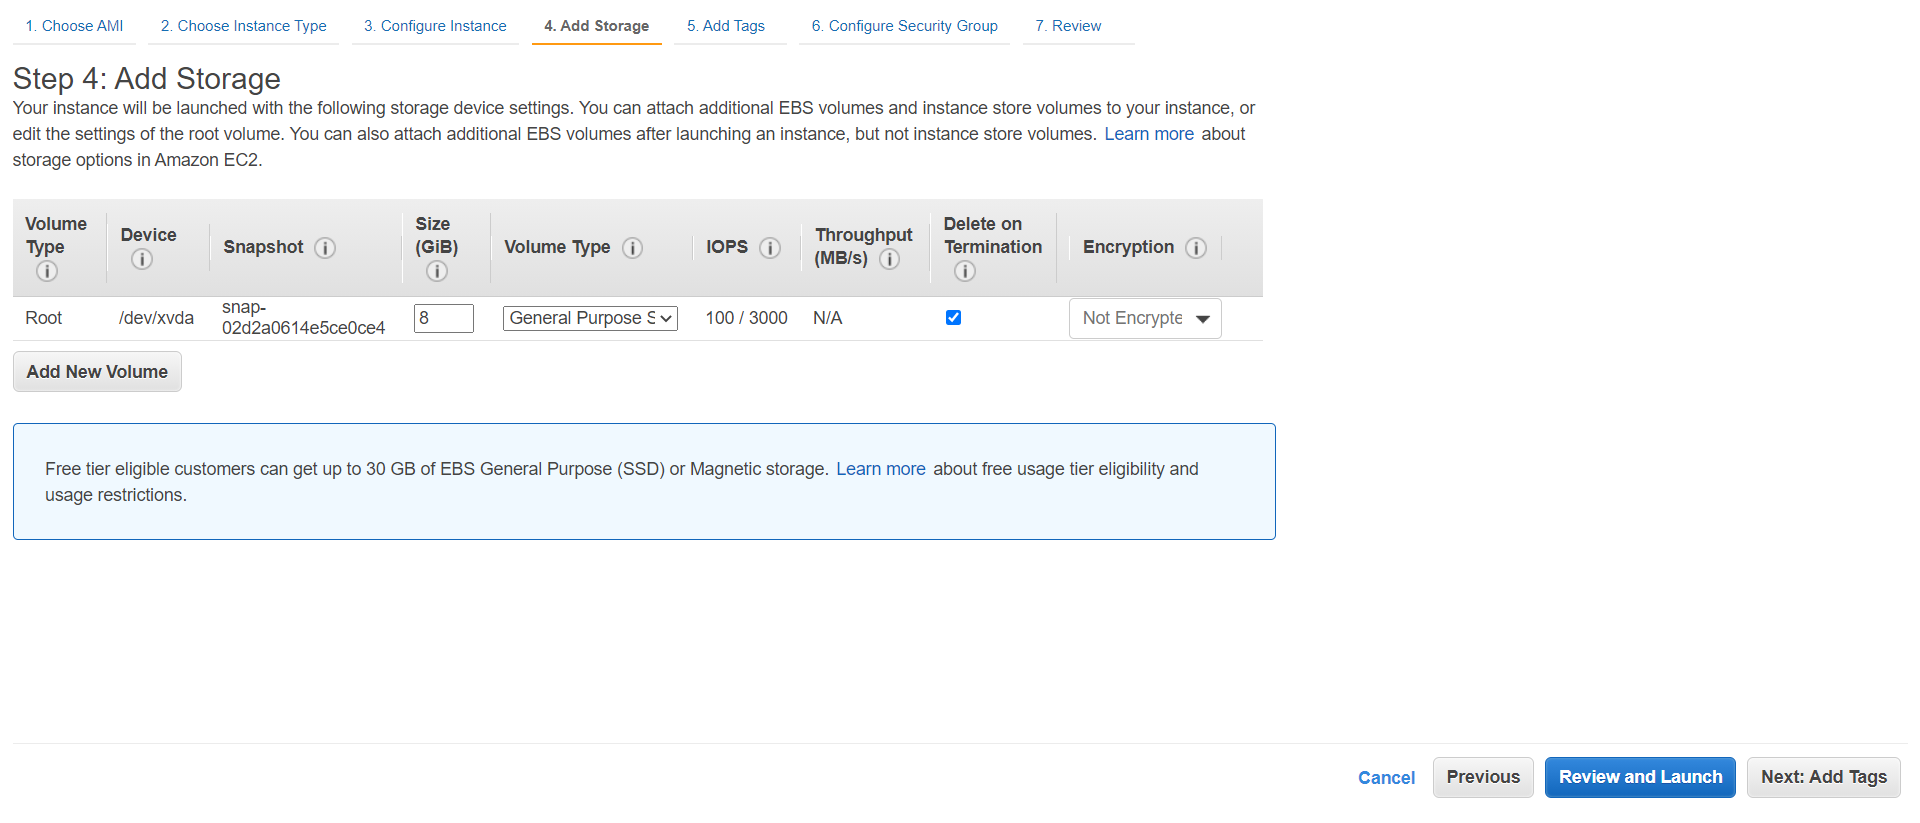
\includegraphics[frame,width=\linewidth]{../Figures/d.png}
    \label{fig:d}
    \caption{Add Storage}
\end{figure}
This is the fourth step in creation of an \acrshort{ec2} instance. This step involves configuration of the storage settings that determine the \acrshort{ebs} volumes used by the launched instance. Instance store volumes are also selected and attached in this step, which is a must since instance store volumes can't be attached after launching the instance. Root directory can also be edited in this step while launching an \acrshort{ec2} instance.


\subsection{Add Tags}
\begin{figure}[H]
    \centering
    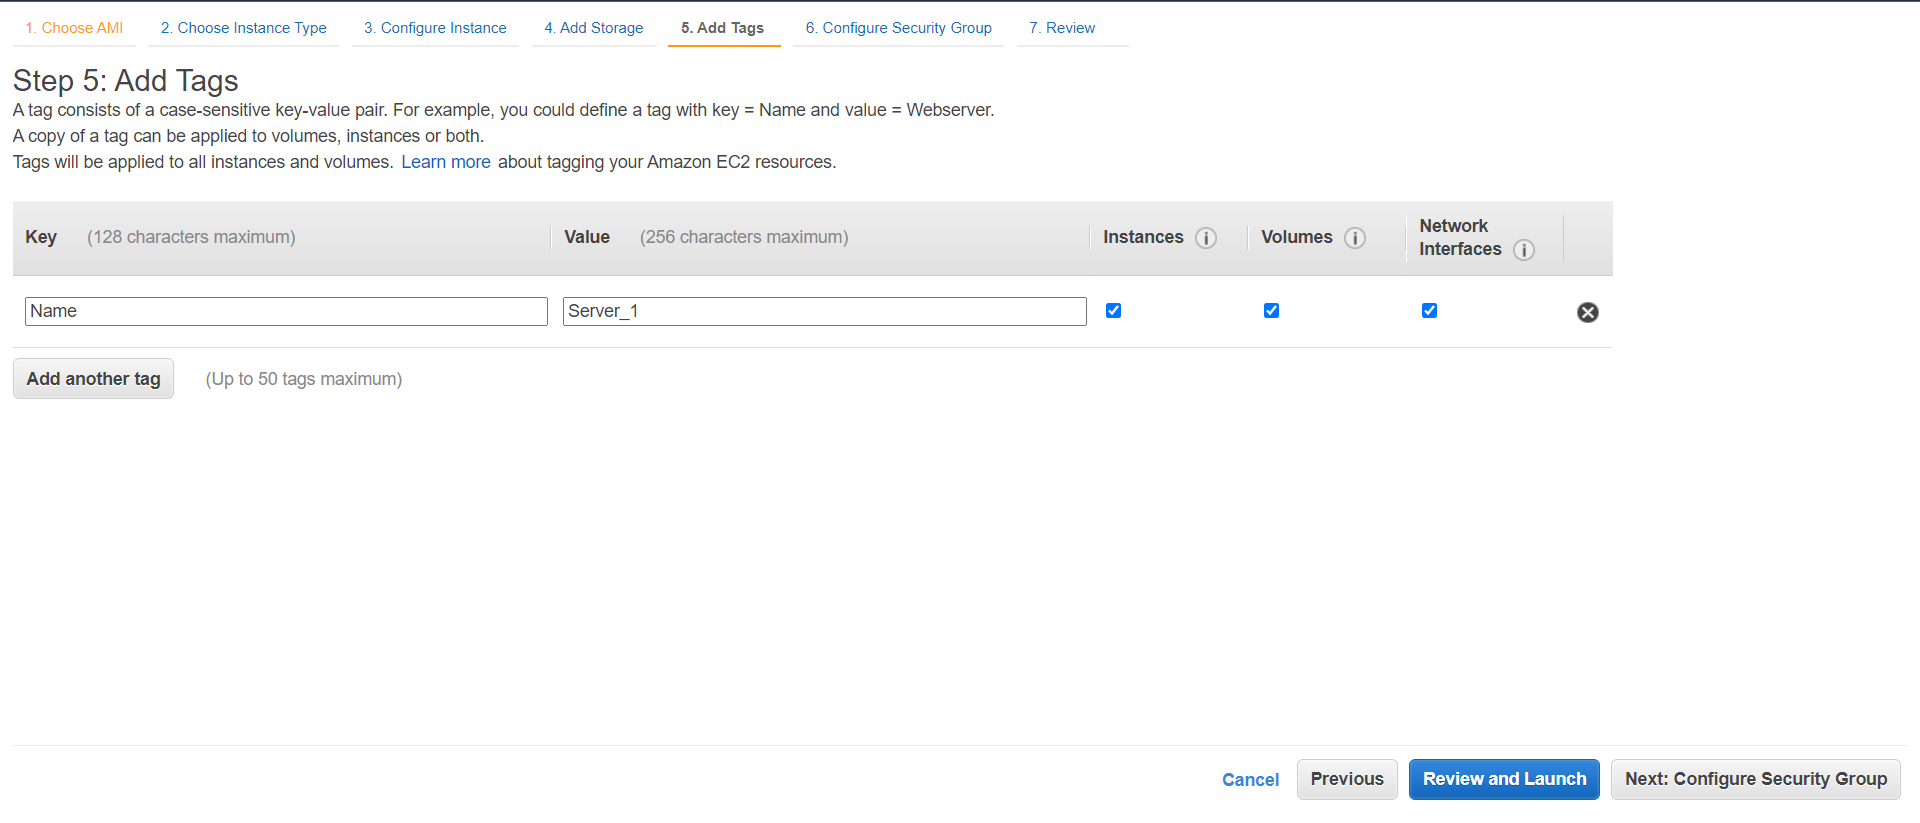
\includegraphics[frame,width=\linewidth]{../Figures/e.png}
    \label{fig:e}
    \caption{Add Tags}
\end{figure}
This is the fifth step in creation of an \acrshort{ec2} instance. This step involves adding or editing tags for the instance. Tags are nothing but key-value identifer pair used to filter the launched instances. For this example, a \textit{Name} tag with the value \textit{Server\_1} is created. This tag is associated to all instance, volume and the used network interfaces.
 
\subsection{Configure Security Groups}
\begin{figure}[H]
    \centering
    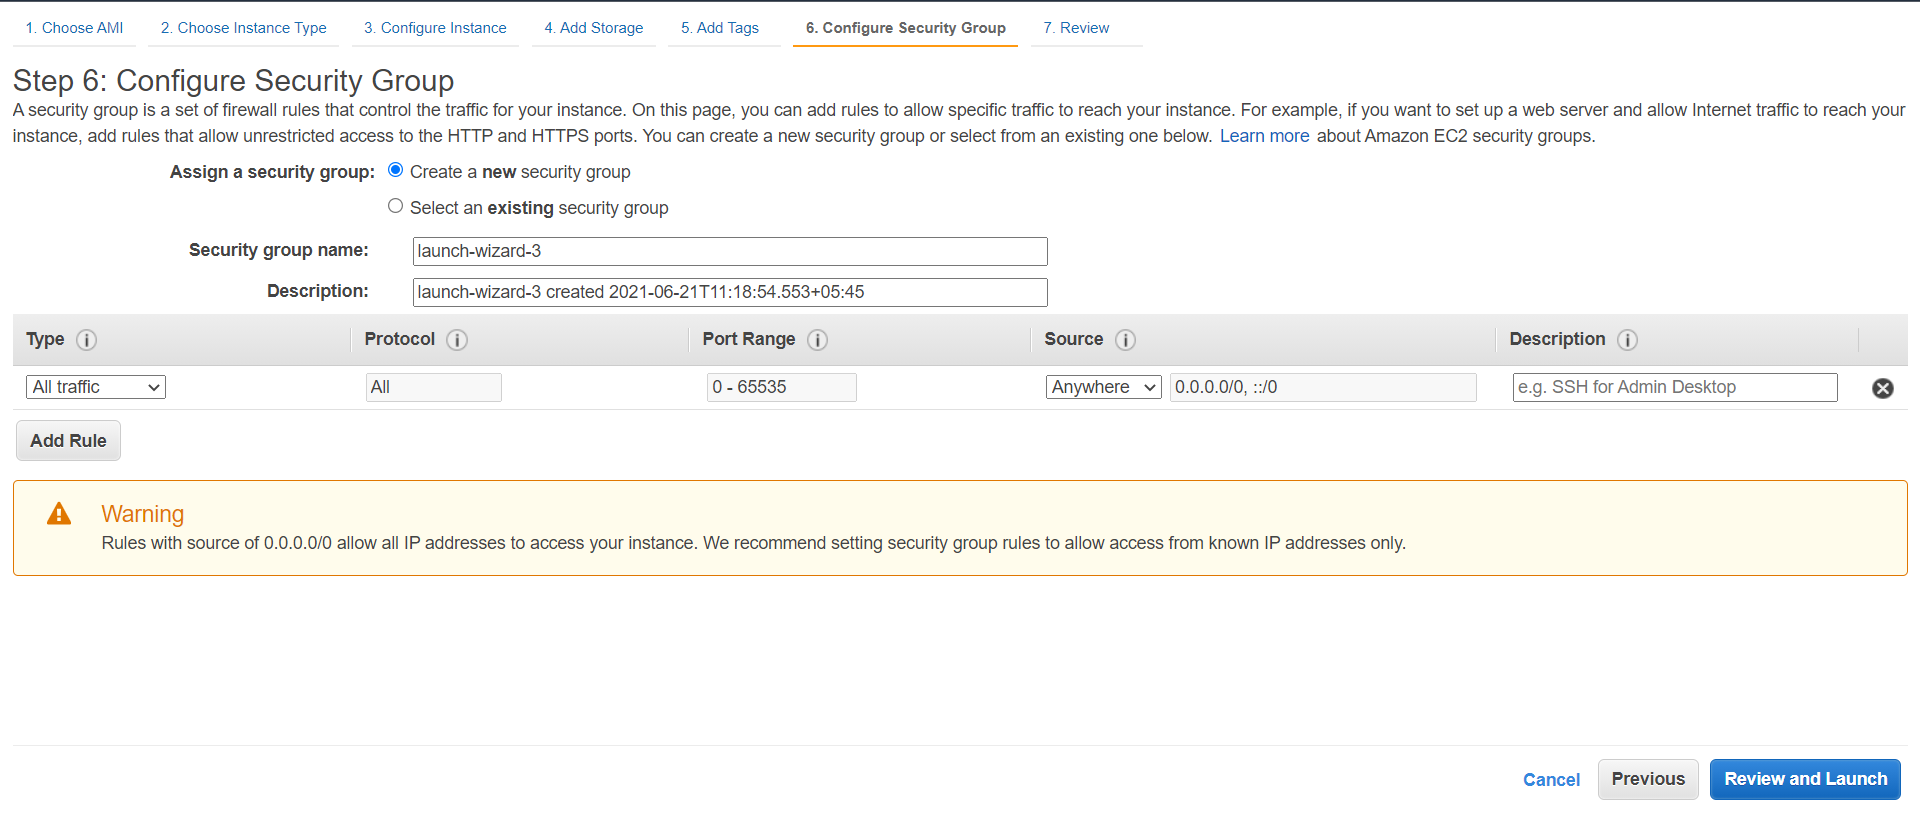
\includegraphics[frame,width=\linewidth]{../Figures/f.png}
    \label{fig:f}
    \caption{Configure Security Groups}
\end{figure}
This is the sixth step in creation of an \acrshort{ec2} instance. This step involves configuration of security groups that are essentially act as firewall to control the inbound traffic to the launched instances. The rules can be set for different traffic types, to follow various communication protocols, use the required port ranges accordingly and source address. For this example, all traffic is allowed for requests coming from any address on the internet. This is obviously not the recommended setting since security will be compromised. 

\subsection{Review and Launch}
\begin{figure}[H]
    \centering
    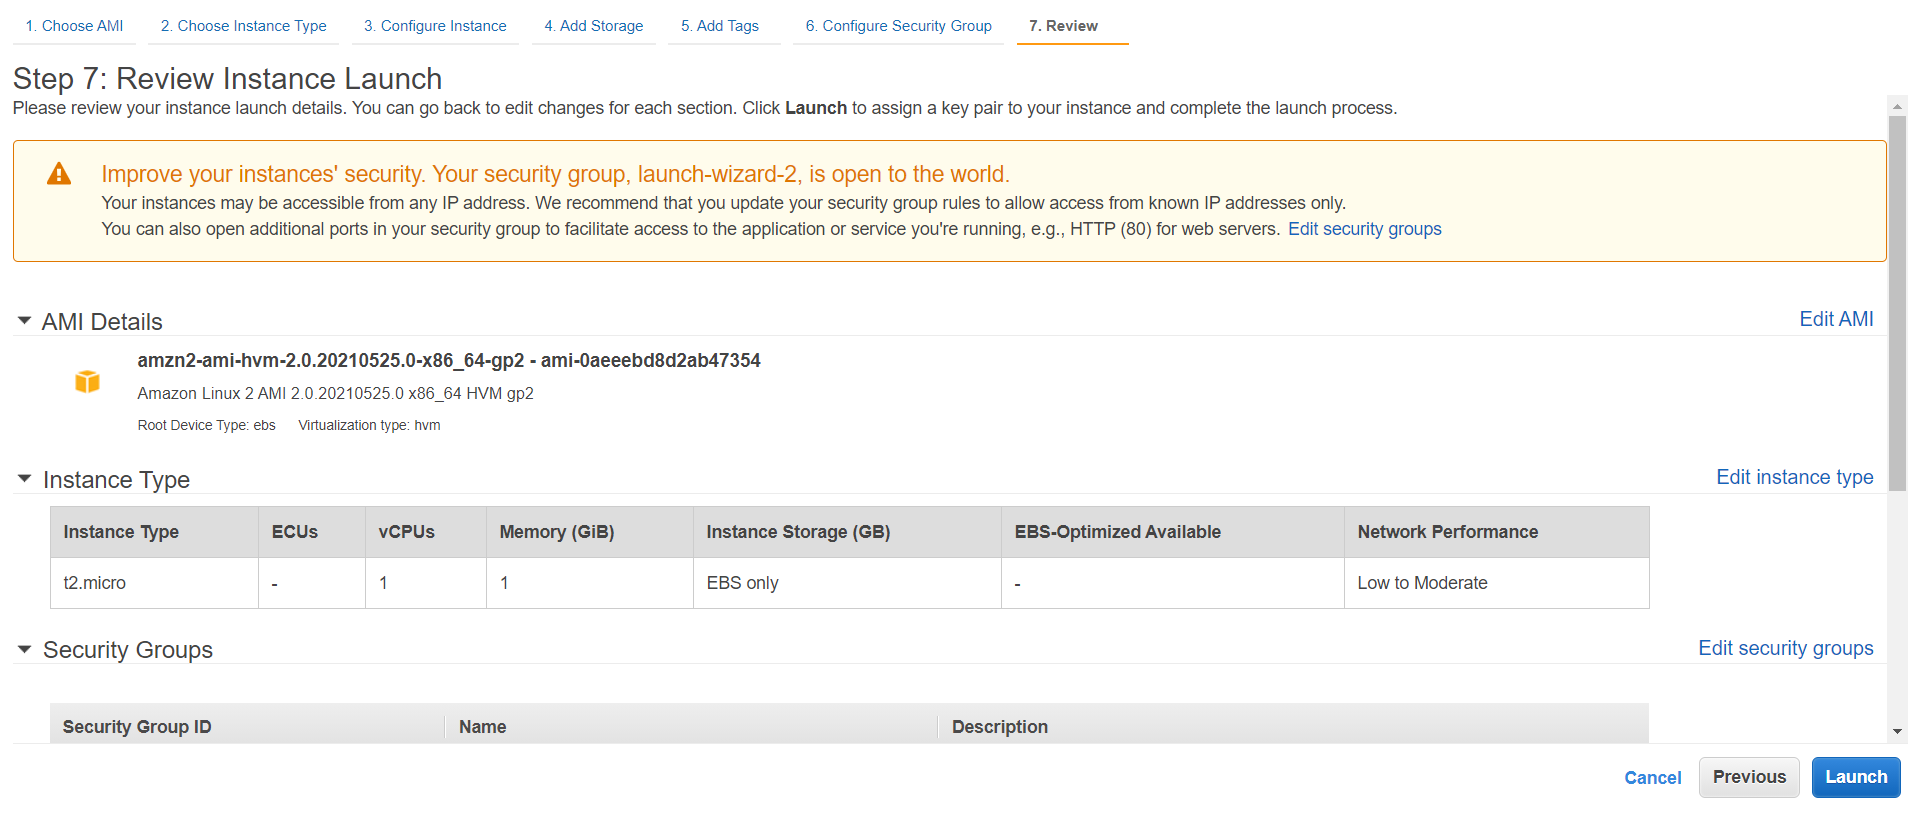
\includegraphics[frame,width=\linewidth]{../Figures/g.png}
    \label{fig:g}
    \caption{Review and Launch}
\end{figure}

This is the seventh and final step in creation of an \acrshort{ec2} instance. This step involves reviewing the set configurations in step 1 to 6 and launching the instance. While launching the instance, clients are recommended to use an existing key pair or generate a new one, that is an encrypted key used for remote access. Once launched the instance will take some time to clear the different status checks.
\end{document}
